\documentclass{report}
\usepackage[utf8]{inputenc}
\usepackage{blindtext}
\usepackage[T1]{fontenc}
\usepackage{graphicx}
\usepackage[
	a4paper,
	left=20mm,
    top=20mm,
    ]{geometry}
\usepackage{hyperref}
\usepackage{amsthm}
\usepackage{enumitem,amssymb}
\usepackage{amsmath}
\usepackage{stackengine}
\usepackage{enumitem}
\usepackage{mathtools}
\usepackage{wrapfig}
\usepackage{multicol}
\usepackage{titlesec}
    \titleformat{\chapter}[hang] 
    {\normalfont\huge\bfseries}{\chaptertitlename\ \thechapter:}{1em}{} 
\graphicspath{ {assets/} }

% ==================
% Custom Functions
% ==================
\newlist{choices}{enumerate}{1}
\setlist[choices]{label*=(\Alph*)}
\newcommand{\choice}{\item}

\hypersetup{
    colorlinks=true,
    linkcolor=blue,
    filecolor=blue,      
    urlcolor=blue,
    }
    
\SetEnumitemKey{twocol}{
  before=\raggedcolumns\begin{multicols}{2},
  after=\end{multicols}}

\SetEnumitemKey{threecol}{
  before=\raggedcolumns\begin{multicols}{3},
  after=\end{multicols}}

\newcommand\kufss{
	\begin{enumerate}[itemsep=15pt,label=,leftmargin=0.5cm]
		\item \textbf{Knowns:}
		\item \textbf{Unknowns:}
		\item \textbf{Formula:}
		\item \textbf{Substitute:}
		\item \textbf{Solve + Unit:}
	\end{enumerate}
}

\newlist{nwa}{itemize}{2}
\setlist[nwa]{label=$\square$}

% ==================
% Set Up Title Page
% ==================
\title{
    \centerline{
\includegraphics[width=50mm]{lymphad.jpg}}
    \vspace{0.5cm}
    Year 12 Physics - Mechanics\\
    \vspace{0.5cm}
    \large AS91171 \\ https://putaiao.nz/12phy/as91171/\\}
    \author{Finn Le Sueur of Cashmere High School\\ \texttt{lsf@cashmere.school.nz}}
    \date{\the\year{}
}

\begin{document}

\maketitle

\newpage

\setcounter{tocdepth}{1}
\tableofcontents

% ====================
%  Speed and Acceleration
% ====================
\newpage
\chapter{Speed and Acceleration}

\section{Warm Up}

\section{Formula: Average Speed}

\subsection{Pātai}

Ash runs $315m$ in $45s$. Calculate his average speed in \textit{meters per second}.

\kufss

\newpage
\chapter{Vectors and Scalars}

\newpage
\chapter{Kinematic Equations}

\newpage
\chapter{Newton's Laws}

\newpage
\chapter{Projectile Motion}

\newpage
\chapter{Torque and Equilibrium}

\newpage
\chapter{Circular Motion}

\newpage
\chapter{Momentum and Impulse}

\newpage
\chapter{Springs}

\newpage
\chapter{Energy, Work, and Power}

\section{Ngā Whāinga Ako}

\begin{nwa}
    \item Be able to calculate gravitational potential energy
    \item Be able to calculate kinetic energy
    \item Be able to use the law of conservation of energy
    \item Be able to define and calculate work
    \item Be able to define and calculate power
\end{nwa}

\begin{align*}
	W &= Fd & E_{k} &= \frac{1}{2}mv^{2} & E_{p} &= mg\Delta h & P &= \frac{W}{t}
\end{align*}

\section{Energy}

Energy is a quantity that must be transferred (transformed) to do \textbf{work}. Here are some types of energy. In Mechanics we are mostly interested in the ones that are \textbf{bolded}.

\begin{itemize}[twocol]
	\item Light
    \item \textbf{Heat}
    \item \textbf{Sound}
    \item Electrical
    \item Radiation
    \item \textbf{Kinetic}
    \item Nuclear potential
    \item Chemical potential
    \item \textbf{Gravitational potential}
    \item \textbf{Elastic potential}
\end{itemize}

\subsection{Unit of Energy}

\begin{itemize}
	\item \textbf{Pātai:} What is the unit for energy?
	\item \textbf{Whakatika:}
\end{itemize}

\section{Kinetic Energy}

The energy that a moving object has. Related to its velocity and mass.

\begin{align*}
    E_{k} &= \frac{1}{2}mv^{2} \\
    E_{k} &= \\
    m &= \\
    v &=
\end{align*}

\subsection{Pātai}
A student is testing how kinetic energy can vary between objects and velocities. He starts by rolling a toy car of mass $50g$ down a hill. It reaches a top speed of $3ms^{-1}$. Calculate its kinetic energy.
\kufss

He then rolls a toy truck down the hill. It reaches $3ms^{-1}$ but has a mass of $100g$. Calculate its kinetic energy.
\kufss

He then finds a steeper hill where his $45g$ car reaches a speed of $9ms^{-1}$. Calculate and compare this kinetic energy with the other two. Which component has a greater impact, mass or velocity?
\kufss
\vspace{3cm}

\section{Gravitational Potential Energy}
Energy an object has by being displaced from \textit{ground} in a gravitational field. Related to its mass and height. Unlike kinetic energy, gravitational potential energy has equal weighting on both mass, acceleration due to gravity and height.

\begin{align*}
    E_{p} &= mg \Delta h \\
    E_{p} &= \\
    m &= \\
    g &= \\
	h &= 
\end{align*}

\subsection{Pātai}
A student with mass $55kg$ climbs a $7.5m$ diving board. Calculate their gravitational potential energy at the top of the diving board.
\kufss

\section{Law of Conservation of Energy}

Energy can neither be created nor destroyed, it can only be \textit{transformed} or \textit{transferred}. This tells us that: \textbf{the total energy in the system is always conserved.} The system might be a collision/explosion, a beaker, Earth or the whole Universe!
To be able to do Physics with this law, we need to state it as an equation. In words we can say, \textit{energy before is equal to energy after}.

\begin{align*}
	E_{i} = E_{f}
\end{align*}

We can also say \textit{in an ideal world all energy is transformed, and none is lost via friction in the form of heat/light}. We understand that in reality this is not the case, but this assumption makes our calculations easier.

For example, when an object falls from a height, its \textit{gravitational potential energy} is transformed into \textit{kinetic energy}, but the total energy in the system is \textit{constant}. In an ideal world 100\% of the energy is transformed from $E_{p}$ to $E_{k}$. Therefore when comparing an object at the top of its fall, to the bottom of its fall we can say:

\begin{align*}
	E_{k} &= E_{p} \\
	\frac{1}{2}mv^{2} &= mgh
\end{align*}

\subsection{Whakakite: Skate Park Simulation}

Open this URL to view the simulation: \url{https://phet.colorado.edu/sims/html/energy-skate-park/latest/energy-skate-park_en.html}

\begin{itemize}
    \item For example, in this simulation, the skater will never go higher than they started.
    \item This is because they cannot \textit{get} extra energy from the surroundings.
    \item In a frictionless world, they will also reach the same height because no energy is lost to the surroundings!
\end{itemize}

\subsection{Pātai: Diving Board}
\begin{wrapfigure}{r}{0.25\textwidth}
	\vspace{-1cm}
    \begin{center}
    	% Sourced from https://app.wizer.me/preview/5UDJWP
    	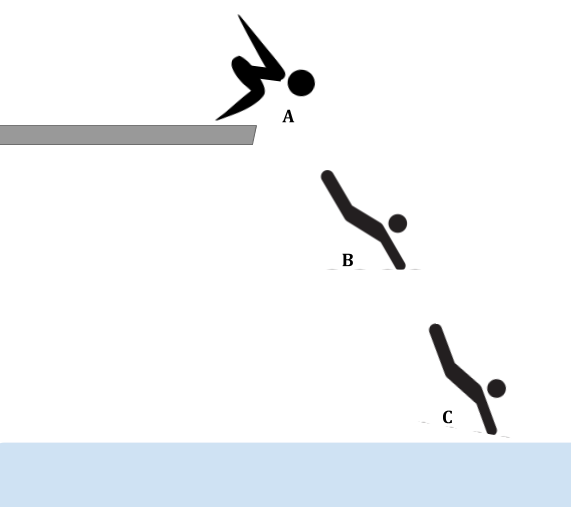
\includegraphics[width=0.9\linewidth]{conservation-of-energy-diving-board.png}
        \label{default}
    \end{center}
\end{wrapfigure}
Think back to the gravitational potential energy diving board question. In an ideal world, all of their gravitational potential energy will be converted to kinetic energy as they fall to the water. In reality some energy will be transferred to heat/sound via air resistance. \textbf{Describe the mixture of kinetic/gravitation energies at A, B and C.}

\begin{enumerate}[label=(\Alph*),itemsep=10pt]
	\item
	\item
	\item
\end{enumerate}

\textbf{Calculate the maximum speed that the diver will reach}.
\kufss

\subsection{Pātai: Bullet and Sandbag}
A bullet of mass $30g$ is fired with a speed of $400ms^{-1}$ into a sandbag. The sandbag has a mass of $10kg$ and is suspended by a rope so that it can swing. \textbf{Calculate the maximum height that the sandbag rises as it recoils with the bullet lodged inside.}

\textbf{Step 1.} Calculate the kinetic energy of the bullet

\kufss

\textbf{Step 2.} Equate this with the potential energy of combined sandbag + bullet

\kufss

\section{Practice}

\begin{itemize}
	\item Homework Booklet: 
	\item Textbook: 
	\item Worksheet: 
\end{itemize}

\section{Work}

\begin{wrapfigure}{r}{0.4\textwidth}
    \vspace{-1cm}
    \begin{center}
    	% Sourced from https://en.wikipedia.org/wiki/Conservative_force
    	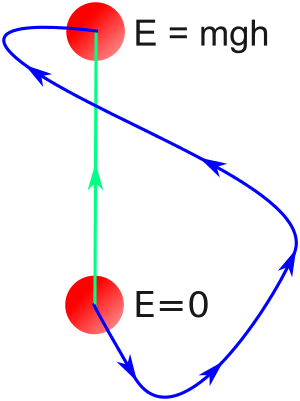
\includegraphics[width=0.9\linewidth]{work-path-independence.png}
        \caption{Path Independence of Energy.}
        \label{default}
    \end{center}
\end{wrapfigure}

Work is defined as \textit{the amount of energy transferred or transformed}. Work is an \textit{amount} of energy, and therefore has the same unit: Joules (J). An important part of work is that it is \text{path independent}. Only the start and end points matter, what happens in the middle does not.

\begin{align*}
	W &= Fd \\
	W &= \\
	F &= \\
	d &=
\end{align*}

\newpage
\section{Power}

\appendix

\chapter{Formula Sheet}

\begin{align*}
    v &= \frac{\Delta d}{\Delta t} & a &= \frac{\Delta v}{\Delta t} \\ \\ \\ \\
    v_{f} &= v_{i}+at & d &= v_{i}t + \frac{1}{2}at^{2} & d &= \frac{v_{i} + v_{f}}{2}t & v_f^{2} &= v_{i}^{2} + 2ad \\ \\ \\ \\
    F_{c} &= \frac{mv^{2}}{r} & a_{c} &= \frac{v^{2}}{r} \\ \\ \\ \\
    p &= mv & \Delta p &= F\Delta t\\ \\ \\ \\
    W &= Fd & E_{k} &= \frac{1}{2}mv^{2} & E_{p} &= mg\Delta h & P &= \frac{W}{t} \\ \\ \\ \\
    F &=ma & \tau &= Fd \\ \\ \\ \\
    E_{p} &= \frac{1}{2}kx^{2} & F &= -kx
\end{align*}


\end{document}
